\chapter{Results and Discussion}
The $v_2$ measurement for \pau \sqsn = 200 GeV $0-5\%$ centrality completes the set of flow measurements in the small systems available at RHIC: \pau, \dau, and \hau. The goal of this set of measurements is to determine the effect of varying initial collision conditions on the resulting flow.
\section{$v_2$ Measurement}
The resulting $v_2$ measurement for p+Au \sqsn = 200 GeV $0-5\%$ centrality is shown in \ref{fig:pau_points_alone}.  The systematic uncertainty is very large especially at high $p_T$ and is dominated by non-flow. The fact the non-flow component is so large warrants further discussion. 

\begin{figure}[!ht]
\begin{center}
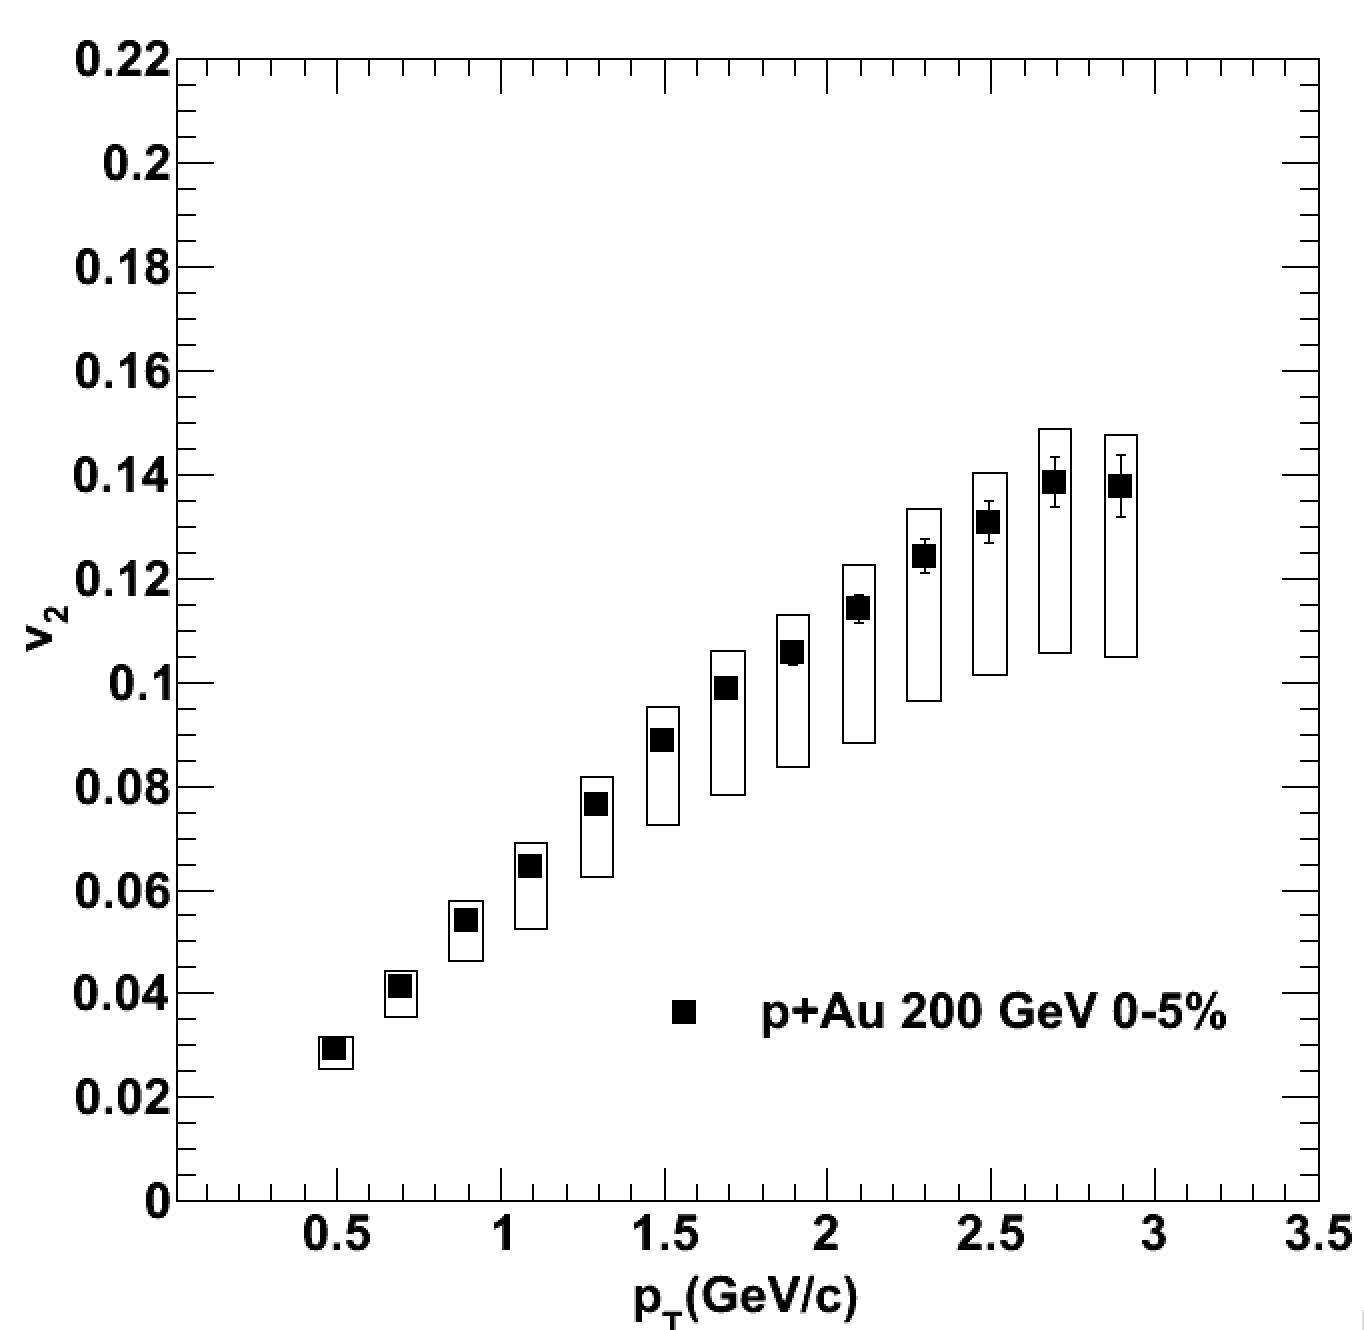
\includegraphics[width=0.65\linewidth]{figs/pau_points.png}
\caption{The $v_2$ measurement of p+Au at \sqsn =  200 GeV 0-5\% centrality.}
\label{fig:pau_points_alone}
\end{center}
\end{figure}

\subsection{Non-flow Contribution}
As was discussed in section .xxx, the non-flow systematic uncertainty can instead be thought of as a systematic error that can be corrected for in our measurement. To further explore this non-flow effect, Figure \ref{fig:pau_points_alone_nf} shows what the p+Au measurement looks like by subtracting the points off the non-flow uncertainty. Due to non-flow being the dominant source of systematic uncertainty, the corrected p+Au points are at the bottom of the systematic uncertainty boxes of the uncorrected points.  The substantial changes this correction makes to the \pau points, especially at high \pt, must be put in context of the field of heavy ion physics. This procedure to estimate the contribution of elementary processes to the measured $v_2$ signal is an attempt at an accurate approximation. Although the non-flow approximation used in this thesis has its merits, there is currently no consensus in the field regarding how to properly quantify how much of the $v_2$ corresponds to ``flow" and how much corresponds to ``non-flow." Other experimental collaborations making flow measurements, such as STAR, ATLAS, and ALICE, treat non-flow in different ways \textbf{TODO add refs for each collab}. Therefore, we choose to explicitly state our methodology to estimate this non-flow and to treat it as a systematic effect that raises the measured $v_2$. %When comparing the \pau points with points from other systems, the non-flow incorporated as a systematic uncertainty.

\begin{figure}[!ht]
\begin{center}
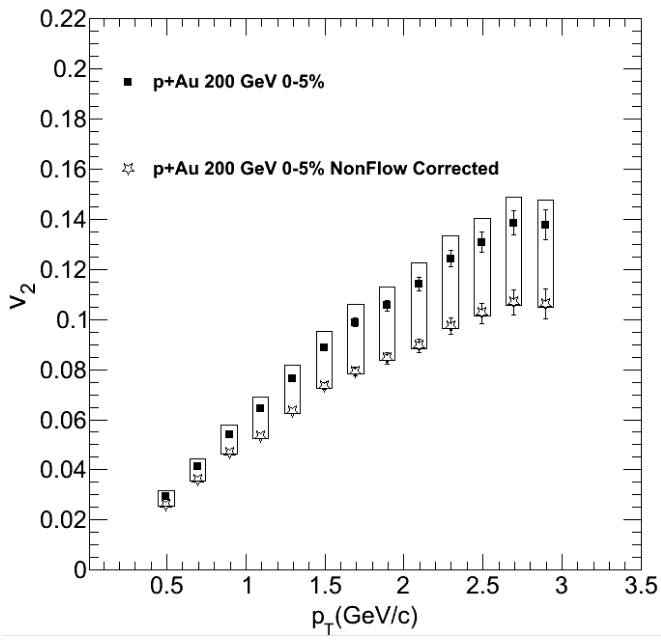
\includegraphics[width=0.65\linewidth]{figs/figure_w_nonflow_corr.png}
\caption{The $v_2$ measurement of p+Au at \sqsn =  200 GeV $0-5\%$ centrality with the statistical and systematic errors corresponding to the bars and the boxes respectively. The stars are the same \pau points but with the non-flow estimate subtracted rather than treated as a systematic uncertainty. \textbf{add ref}}
\label{fig:pau_points_alone_nf}
\end{center}
\end{figure}

%\subsection{$v_2$ vs Multiplicity}
\section{Comparison with Other Species at \sqsn =  200 GeV 0-5\% Centrality}
The substantial $v_2$ p+Au is interesting in itself but the significance of the measurement is best understood by comparing it to other small collision system results, specifically He+Au and d+Au. In order to properly make the strongest physics statement possible in this comparison, we attempt to hold as many variables constant across all three datasets. Table \ref{tbl:species_compare} compares the various relevant parameters for the three collision species. Among the differences across the columns, the largest is the lack of non-flow estimates for the \dau datasets. In the interest of measurement compatibility, and for the reason stated in section .xxx, there is no non-flow correction applied to any of the datasets.

\begin{table}[h!]
\caption{Dataset Variables Comparison listed in order: center of mass energy per nucleon, centrality, mid-rapidity charged particle multiplicity per unit of psuedo-rapidity, year, trigger (as defined in section .xxx) particle sample, trigger particle acceptance, event plane determination, $\Psi_2$ Resolution, condition of available non-flow estimate.}
\begin{center}
    \begin{tabular}{| c | c | c | c |}
    \hline
    Variable & \pau  & \dau & \hau\\ \hline \hline
    \sqsn (GeV) & 200 & 200 & 200\\ \hline
    Centrality & 0-5\%  & 0-5\% & 0-5\% \\ \hline
    Mid-rapidity $dN_{ch}/d\eta$ & N/A & 20.8 +/- 1.5 & 26.3 +/- 1.8 \\ \hline 
    Year (collected) & 2015  & 2008 & 2014 \\ \hline
    Trigger Particle Sample & Charged Hadrons & Charged Hadrons & Charged Hadrons \\ \hline
    Trigger Particle Acceptance & $|\eta| <$ 0.35  & $|\eta| <$ 0.35 & $|\eta| <$ 0.35 \\ \hline
    Event Plane &  -3$<\eta<$-1 (FVTXs) & -3.7$<\eta<$-3.1 (MPCs) &  -3$<\eta<$-1 (FVTXs) \\ \hline
    $\Psi_2$ Resolution & 0.171 & 0.14 & 0.274 \\ \hline %maybe add pt averaged v2?
     Non-flow Estimate& yes & no & yes\\ \hline
     %Glauber $\epsilon_2$ & 0.23 &  0.54 & 0.50\\ \hline
    \end{tabular}
\end{center}
\label{tbl:species_compare}
\end{table}
%\begin{table}[h!]
%\caption{To Do: make systematic error table.}
%\begin{center}
%    \begin{tabular}{c | c | c | c}
%    \hline
%    variable & \pau  & \dau & \hau\\ \hline \hline
%    \sqsn (GeV) & 200 & 200 & 200\\ \hline
%    \end{tabular}
%\end{center}
%\end{table}
% discuss centrality selections between the different measurements
% maybe show the multiplicity matched plot? would have to accurately explain caveats NO
Figure  \ref{fig:v2_3_sys_compare_nohydro} shows the $v_2(p_T)$ measurements in the three systems. All three measurements exhibit substantial $v_2$ values and rise as a function of $p_T$ with a similar shape. The error bars of each measurement indicate the rough equivalence of the He+Au and d+Au measurements relative to the p+Au measurement. In fact, the systematic error bars are large enough for the p+Au that the difference between p+Au and the other two systems maybe even larger. This effect is especially clear at low $p_T$, where bulk effects would be most dominant. In order to understand the significance of this set of measurements, comparison to standard theoretical models are useful.

\begin{figure}[!ht]
\begin{center}
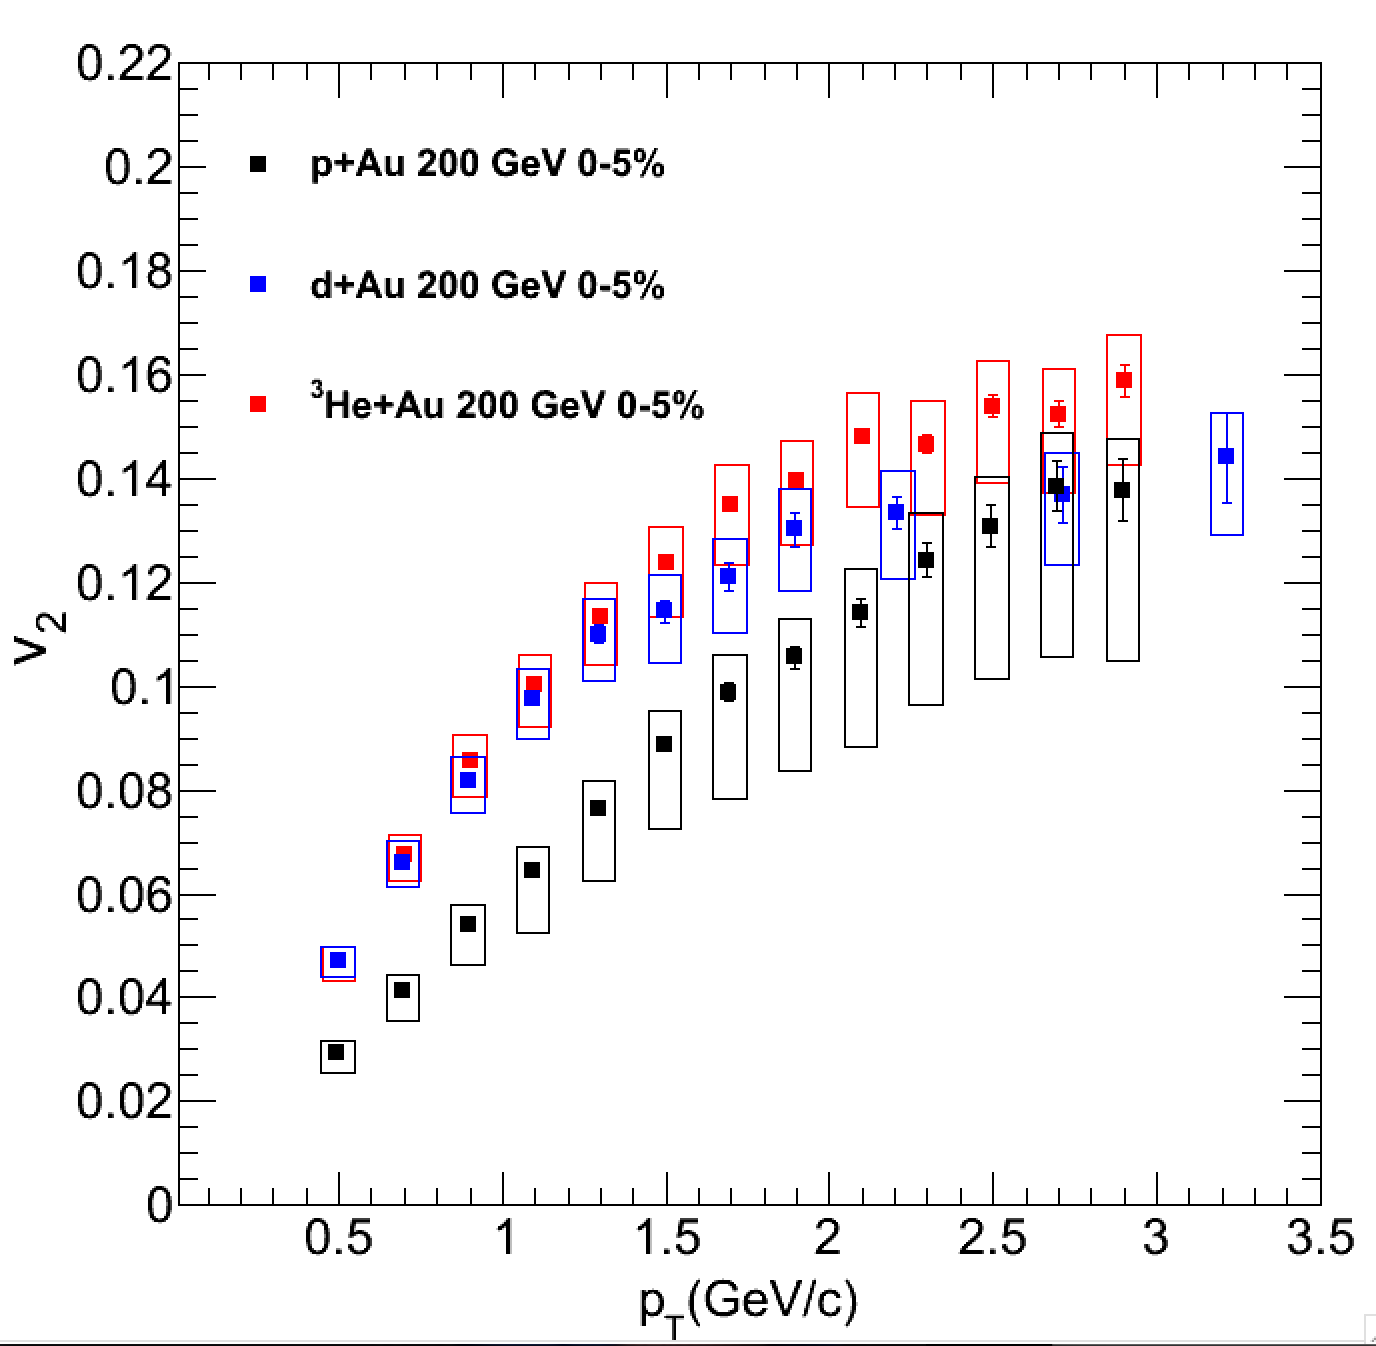
\includegraphics[width=0.65\linewidth]{figs/v2_3_sys_compare_nohydro.png}
\caption{$v_2$ of charged hadrons within $|\eta| <$ 0.35 in 0-5\% p+Au compared to calculations using the \textsc{sonic} model match to the same multiplicity as the data. The model calculations have good agreement with the center of the systematic uncertainty bars.}
\label{fig:v2_3_sys_compare_nohydro}
\end{center}
\end{figure}

\section{Comparison with Theory}

%\subsection{SONIC}
Also shown in Figure ~\ref{fig:all_system_hydro} are $v_2$ calculations for each system from the SONIC hydrodynamic model~\cite{Habich:2014jna}, which incorporates standard Monte Carlo Glauber initial conditions followed by viscous hydrodynamics with $\eta/s=0.08$, and a transition to a  hadronic cascade at $T=$ 170 MeV. More on the SONICE hydrodynamic model is described in greater detail in Chapter 2. It is notable that these calculations for each system are matched to the charged particle density at midrapidity, with the exact values for 0-5\% centrality of 10.0, 20.0, and 27.0, for p+Au, d+Au, and He+Au collisions, respectively~\cite{Habich:2014jna}. As mentioned above, the $dN_{cn}/d\eta$ has not been measured for p+Au, and the value of 10.0 was extrapolated from measurements in the other two systems~\cite{Habich:2014jna}. Thus, we see that the calculation includes both the geometry-related change in eccentricity and the relative collision multiplicity. In all cases, a good agreement is seen within the uncertainties between the data and the calculation. These observations strongly support the notion of initial geometry coupled to the hydrodynamic evolution of the medium as a valid framework to understand small system collectivity.

%\begin{figure}[!ht]
%\begin{center}
%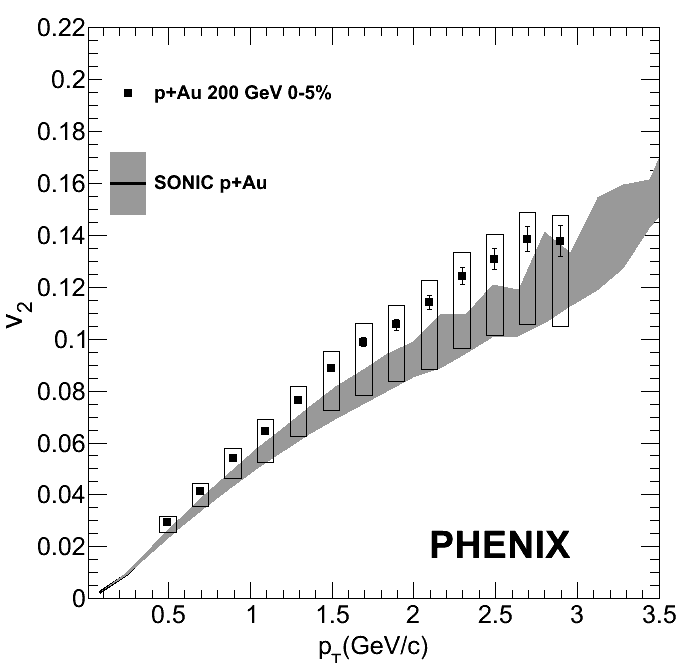
\includegraphics[width=0.65\linewidth]{figs/pau_sonic_alone.png}
%\caption{$v_2$ of charged hadrons within $|\eta| <$ 0.35 in 0\%--5\% p+Au compared to calculations using the \textsc{sonic} model match to the same multiplicity as the data. The model calculations have good agreement with the center of the systematic uncertainty bars.}
%\label{fig:hydro_pau_alone}
%\end{center}
%\end{figure}

\begin{figure}[!ht]
\begin{center}
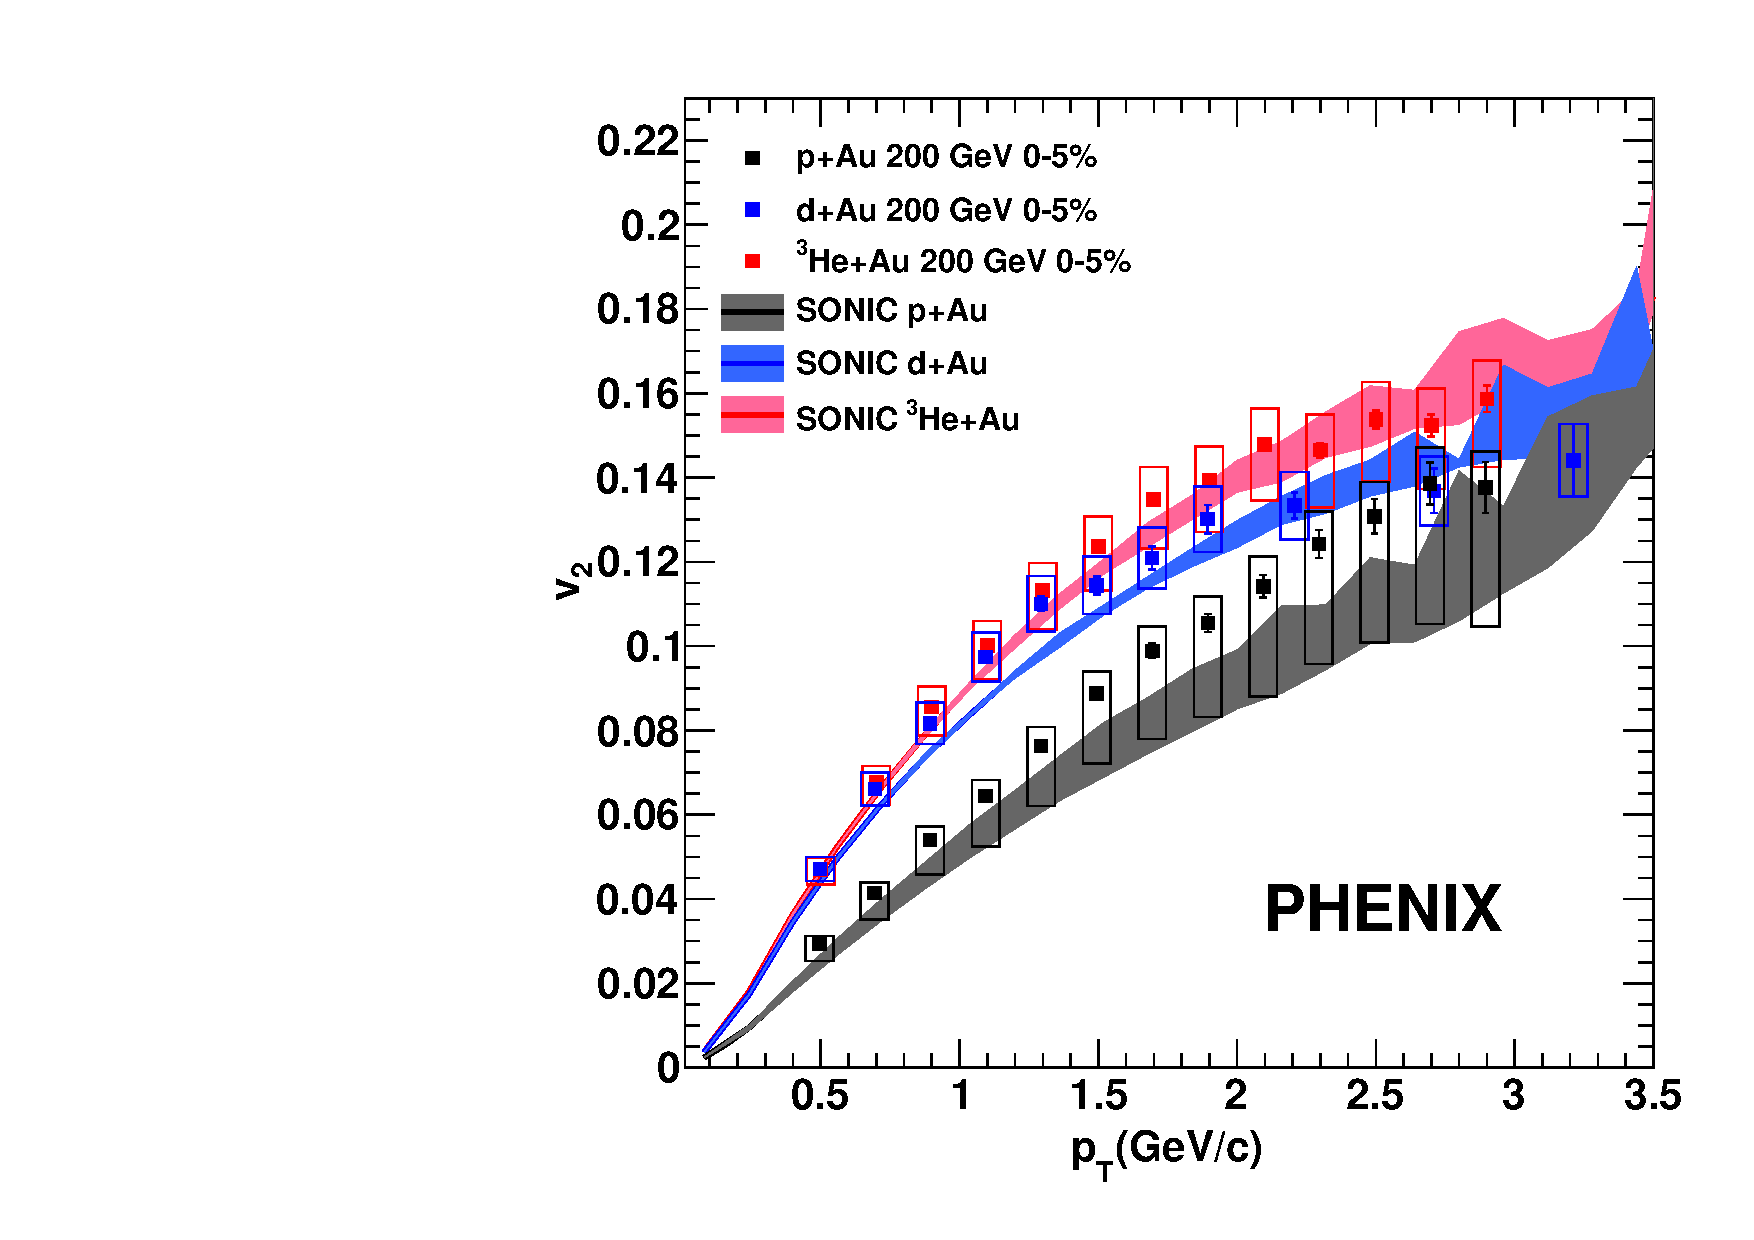
\includegraphics[width=0.65\linewidth]{figs/three_system_comparison_result.png}
\caption{$v_2$ of charged hadrons within $|\eta| <$ 0.35 in 0-5\% p+Au, d+Au, and He+Au central collisions, compared to hydrodynamic calculations using the \textsc{sonic} model, matched to the same multiplicity as the data. Note that the data points shown include non-flow contributions, whose estimated magnitude is accounted for in the asymmetric systematic uncertainties.}
\label{fig:all_system_hydro}
\end{center}
\end{figure}

To further explore this idea, we divide the $v_2$ curves by their corresponding $\epsilon_2$ from Table \ref{tbl:species_compare}, attempting to establish
 a scaling relation between the two quantities. Figure \ref{fig:v2_divided_epsilon_all_sys} shows that the ratios do not collapse to a common value. As
 expected, this behavior is also reproduced by the SONIC calculation, because both data and calculation are divided
 by the same $\epsilon_2$ values. The lack of scaling in the sonic calculation can be understood from d+Au events where
 the neutron and proton from the deuteron projectile are far separated and create two hot spots upon impacting the 
Au nucleus, as seen in Figure \ref{fig:v2_epsi2_ampt}. These events have a large $\epsilon_2$, but can result in small $v_2$ if the two hot spots evolve separately, never
combining within the hydrodynamic time evolution. This effect is present in the d+Au and He+Au systems, and lowers the average $v_2$/$\epsilon_2$. 
%as detailed in Ref. [18].
\begin{figure}[!ht]
\begin{center}
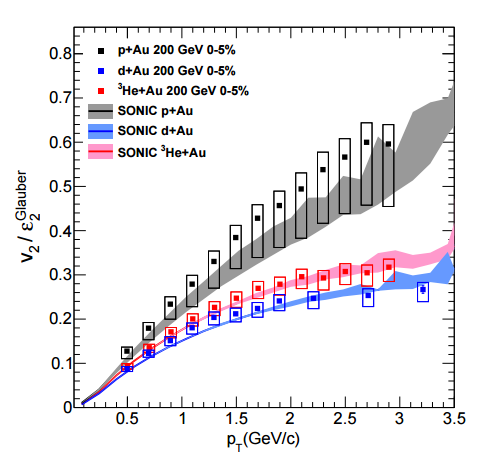
\includegraphics[width=0.65\linewidth]{figs/v2_divided_epsilon_all_sys.PNG}
\caption{$v_2$ of charged hadrons within $|\eta|$ $<$ 0.35 in 0–5\% p+Au,  d+Au, and He+Au central collisions, divided by their corresponding eccentricity $\epsilon_2$ from Glauber calculations, compared to sonic calculations of the same quantity. Note that the data points shown include non-flow contributions, whose estimated
magnitude is accounted for in the asymmetric systematic uncertainties.}
\label{fig:v2_divided_epsilon_all_sys}
\end{center}
\end{figure}

\subsection{Initial Conditions and Eccentricity}
In order to better understand the comparison of the three systems, a deeper understand of the initial conditions is warranted. One critical quantity to characterize the initial collision symmetry is known as the eccentricity. The second order eccentricity, $\epsilon_2$, can be calculated from the distribution of the nucleons involved in the initial collision as:

\begin{equation}
\epsilon_2 = \frac{\sqrt{<r^2 \cos(2\phi)>^2+<r^2 \sin(2\phi)>^2}}{<r^2>},
\end{equation}

where r is the radial nucleon position relative to the centroid of the participants and $\phi$ is the azimuthal angle of the nucleons.

%+\left<r^2 \sin(2\phi)>\right^2}%/\left<r^2>\right
Figure  \ref{fig:initial_condition_comparison}  shows the spatial symmetries present in initial conditions of the three collision species, as well the as a snap shot of the QGP in mid-evolution.  Where as the eccentricities of d+Au and He+Au collisions are largely based on relative nucleon orientation, the initial condition of p+Au is solely based on the orientation of the lone proton and any fluctuations in the target gold nucleus. This means that the determination of the eccentricity from d+Au and He+Au is much better understood than that of p+Au, and can give insight into the lack of uniformity in Figure \ref{fig:v2_divided_epsilon_all_sys}. Table \ref{tbl:eccentricities} illustrates the uniqueness of the p+Au system by showing the diverging range of $\epsilon_2$ values which can be calculated by different nuclear collision models. In addition to this understanding, the concept of overlapping, expanding hotspots creating substantial final state flow, as seen in section .xxx, shows the relative spatial orientation of the initial hotspots and the symmetry axis of flow, otherwise known as the event plane. For example, in the d+Au collision, the event plane vector is transverse to the line that connects the deuteron's nucleons. 

\begin{figure}[!ht]
\begin{center}
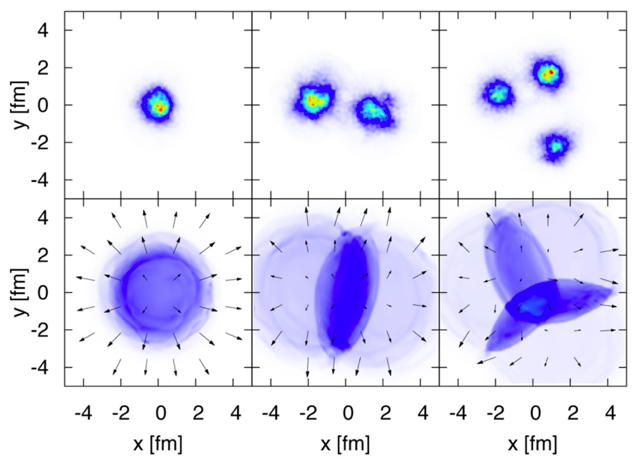
\includegraphics[width=0.75\linewidth]{figs/initial_condition_comparison.png}
\caption{The top three panes show the transverse spatial locations of the initial hot spots of the three collision species, p+Au, d+Au, and He+Au respectively as simulated by Monte Carlo Glauber (?). The bottom three plots show the resulting medium produced from the overlapping hot spots as well as the resulting particle momentum vector field as calculated from hydro (?).\textbf{add ref}}
\label{fig:initial_condition_comparison}
\end{center}
\end{figure}

\begin{table}[h!]
\begin{center}
\caption{Initial eccentricity $\epsilon_2$ of small systems at $\sqrt{s}$ = 200 GeV for $0-5\%$ centrality from Monte Carlo Glauber initial conditions smeared with a two-dimensional Gaussian of width $\sigma=0.4$ fm, and IP-Glasma initial conditions.}
\begin{tabular}{c c c c}
\label{table_geometry_glasma}
 & p+Au & d+Au & He+Au \\ \hline
 Glauber $\langle \varepsilon_2 \rangle$ & $0.23\pm 0.01$ & $0.54\pm 0.04$ & $0.50\pm 0.02$ \\
 IP-Glasma $\langle \varepsilon_2 \rangle$ & $0.10\pm 0.02$ & $0.59\pm 0.01$ & $0.55\pm 0.01$ \\
\label{tbl:eccentricities}
\end{tabular}
\end{center}
\end{table}

Figure \ref{fig:v2_epsi2_ampt} gives an insight into how initial eccentricities, as defined in section xxx., become transformed into final state flow.
The plot was produced by running many events for p+Au,
d+Au, and He+Au systems with different values for the shear
viscosity and the initial spatial distribution smearing.
The final freeze-out hyper-surface of each event is then
translated into a distribution of hadrons via the CooperFrye
freeze-out prescription \textbf{add ref}. In Figure \ref{fig:v2_epsi2_ampt},
the flow coefficients from the different systems and
the scaling between initial spatial $\epsilon_2$ moments and final
state momentum $v_2$ values are compared.
 Figure \ref{fig:v2_epsi2_ampt} shows the pion vn at
$p_T$ = 1.0 GeV/c divided by $\epsilon_2$ as a function of $\epsilon_2$ for each
individual p+Au, d+Au, and He+Au event, for different
freezeout temperatures $T)F$ controlling the lifetime of the
system in the plasma phase. The figure
shows a reasonably common scaling of $v_2/\epsilon_2$ for all three
systems with the d+Au and He+Au simply extending
to larger eccentricities with only a modest dependence
on $T_F$. There are a small set of events with very large
$\epsilon_2$, but have a rather small final $v_2$. Examination of these
events reveals them to be d+Au events where the two
hot spots are so far apart that the hydrodynamic fluids
never connect during the time evolution, as seen in the overlay in Figure \ref{fig:v2:epsi2_ampt}, in order to produce
nearly any elliptic flow. There are a few He+Au in
this category, seen where two nucleons are very close and the
third is quite far away, again having the same effect.

\begin{figure}[!ht]
\begin{center}
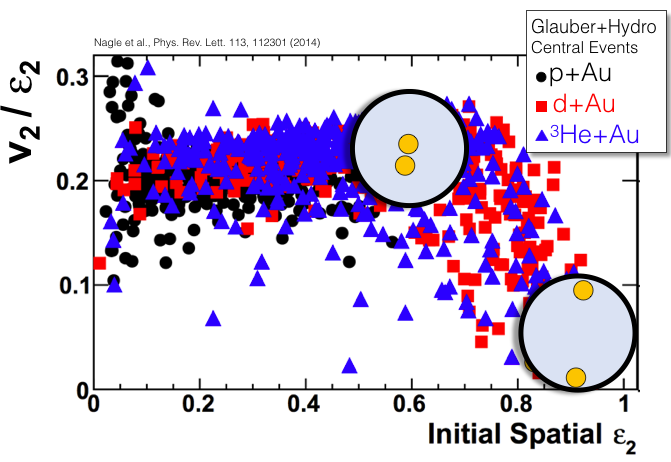
\includegraphics[width=0.6\linewidth]{figs/v2_e2_ampt.png}
\caption{$v_2/\epsilon_2$ versus $\epsilon_2$ with the flow coefficient
for pions evaluated at $p_T$ = 1.0 GeV/c from p+Au,
d+au, and He+Au central (b $<$ 2 fm) events. The results
are with input parameters $\eta$/s = 1/4$\pi$ and initial Gaussian
smearing $\sigma$ = 0.4 fm and a freeze-out temperatures of $T_F$ = 150
MeV. Diagrams of two possible d+Au initial configurations are overlayed on top of the plot. Increasing distance between the two d+Au nucleons correspond to a larger $\epsilon_2$.\textbf{add ref}}
\label{fig:v2_epsi2_ampt}
\end{center}
\end{figure}



Another model that incorporates degrees of freedom extends the Monte Carlo Glauber approach
to also incorporate collisions between constituent quarks . Recently, this framework has been successfully applied
to the description of midrapidity charged particle multiplicity and transverse energy production \textbf{add ref}. Different
implementations of constituent quark Monte Carlo Glauber calculations are detailed in \textbf{add refs}. In Figure 13(f) of
Ref. [12], the initial eccentricities $\epsilon_2$ in p+Au, d+Au, and He+Au obtained by incorporating constituent quarks, in
addition to multiplicity fluctuations, are found to be $\epsilon_2$ = 0.42, 0.54, and 0.54, respectively. This calculation assumes
a Gaussian density distribution of low-x gluons around each constituent quark, of width $\sigma_g$ = 0.3 fm. It is interesting
to note that the d+Au and He+Au systems show little sensitivity to the incorporation of both constituent quarks
 and multiplicity fluctuations into the calculation of the initial $\epsilon_2$. Conversely, under the same circumstances, p+Au
 has a substantially larger $\epsilon_2$ than in the models shown in Table \ref{tbl:eccentricities}. Ref. [13] also presents calculations incorporating
 nucleonic degrees of freedom and multiplicity fluctuations, in which case a lower $\epsilon_2$ = 0.34 is obtained for p+Au. This
 shows that, when compared to the Glauber $\epsilon_2$ for p+Au in Table \ref{tbl:eccentricities}, quark-level degrees of freedom and multiplicity
 fluctuations may both play a significant role. 

\subsection{Comparison to Alternative Models}
Although hydrodynamic models like SONIC are the standard in which elliptical flow is understood in the field of heavy ions, it is important to test the accuracy and consistency of other models against our data. Figure \ref{fig:indepth_comp_three} depicts the established $v_2(p_T)$ data curves with four different model comparisons. Theoretical predictions are
 available in the literature, most notably from hydrodynamics with Glauber initial conditions (SONIC \textbf{add ref} and SUPERSONIC \textbf{add ref}), hydrodynamics with IP-Glasma initial conditions \textbf{add ref}, and A-Multi-Phase-Transport Model (AMPT) \textbf{add ref}.
 The SUPERSONIC model uses the same prescription for initial conditions, hydrodynamic expansion, and hadronic
 cascade as SONIC, yet additionally incorporates pre-equilibrium dynamics with a calculation in the framework of the
 AdS/CFT correspondence \textbf{add ref}.

For the model of IPGlasma+Hydro, in the case of d+Au and He+Au, a better agreement with data can be achieved by increasing the value of $\eta$/s or
by including a hadronic cascade stage. However, doing so would lower the prediction for p+Au even further. This demonstrates that IP-Glasma does not generate the appropriate initial conditions to account for measured $v_2$ via hydrodynamic flow.

 SONIC and SUPERSONIC agree well with the data within uncertainties, supporting the
 idea of initial geometry as the driver of the $v_2$ signal. Furthermore, this illustrates how these results impose useful
 constraints to reduce the number of free parameters of the model, because many such parameters must be identical
 across systems, e.g., $\eta$/s, the transition temperature to a hadron cascade, and the Monte Carlo Glauber smearing of
 nucleon coordinates of $\sigma$ = 0.4 fm.

 Calculations using IP-Glasma initial conditions followed by viscous hydrodynamics have been successfully used to
 describe collectivity in A+A collisions \textbf{add ref}. It is notable that in these calculations the glasma framework is used only
 to determine the initial spatial configuration as input to hydrodynamics; there is no glasma diagram or momentum
 domain physics incorporated, such that all of the collectivity arises from final-state interactions. When this framework
is applied to small collision systems with $\eta$/s = 0.12 and b $<$ 2 fm, as shown in Figure \ref{fig:indepth_comp_three}, the calculation substantially
overestimates the data for d+Au and He+Au, while underestimating it for p+Au. This follows from the fact that
 IP-Glasma generates very circular initial conditions for p+Au, corresponding to very low $\epsilon_2$ values; however, the
presence of several hot spots in d+Au and He+Au result in IP-Glasma values for $\epsilon_2$ more comparable to those from
 Glauber. This is shown in Table \ref{tbl:eccentricities}.

It is important to notice that additional degrees of freedom for the geometry of p+Au collisions arise from fluctuations of the shape of the proton, as described in Ref. \textbf{add ref}. The contribution of this effect to the measured elliptic flow may be constrained by p+p data, and also possibly by varying the target in other p+A systems.

Finally, AMPT, as described in Chapter 2, combines partonic and hadronic scattering in a single model. Central AMPT events with impact parameter $b<2$ have a midrapidity $dN_{ch}/d\eta$ = 8.1, 14.8, and 20.7 for p+Au, d+Au, and He+Au, respectively. These were generated with the same Monte Carlo Glauber initial conditions used to characterize event geometry, and thus have very similar eccentricities to those given in Table \ref{tbl:eccentricities}. Using the initial Glauber geometry information to compute $v_2$ relative to the participant plane~\cite{Koop:2015wea} yields results that agree reasonably well with the data below $\pt \approx 1$ GeV/c, yet under predict them at higher \pt. It is noteworthy that despite the very different physics of AMPT compared to the other models, it has successfully been applied to a variety of systems at RHIC and the LHC \textbf{add refs}. 
%See, for example, \textbf{add refs}. 
%Refs.~\cite{Adare:2015cpn,Koop:2015wea,Ma:2016fve,ma_long-range_2014,ma_long-range_2014}

%\subsection{IP-Glasma with Hydro}
\begin{figure}[!ht]
\begin{center}
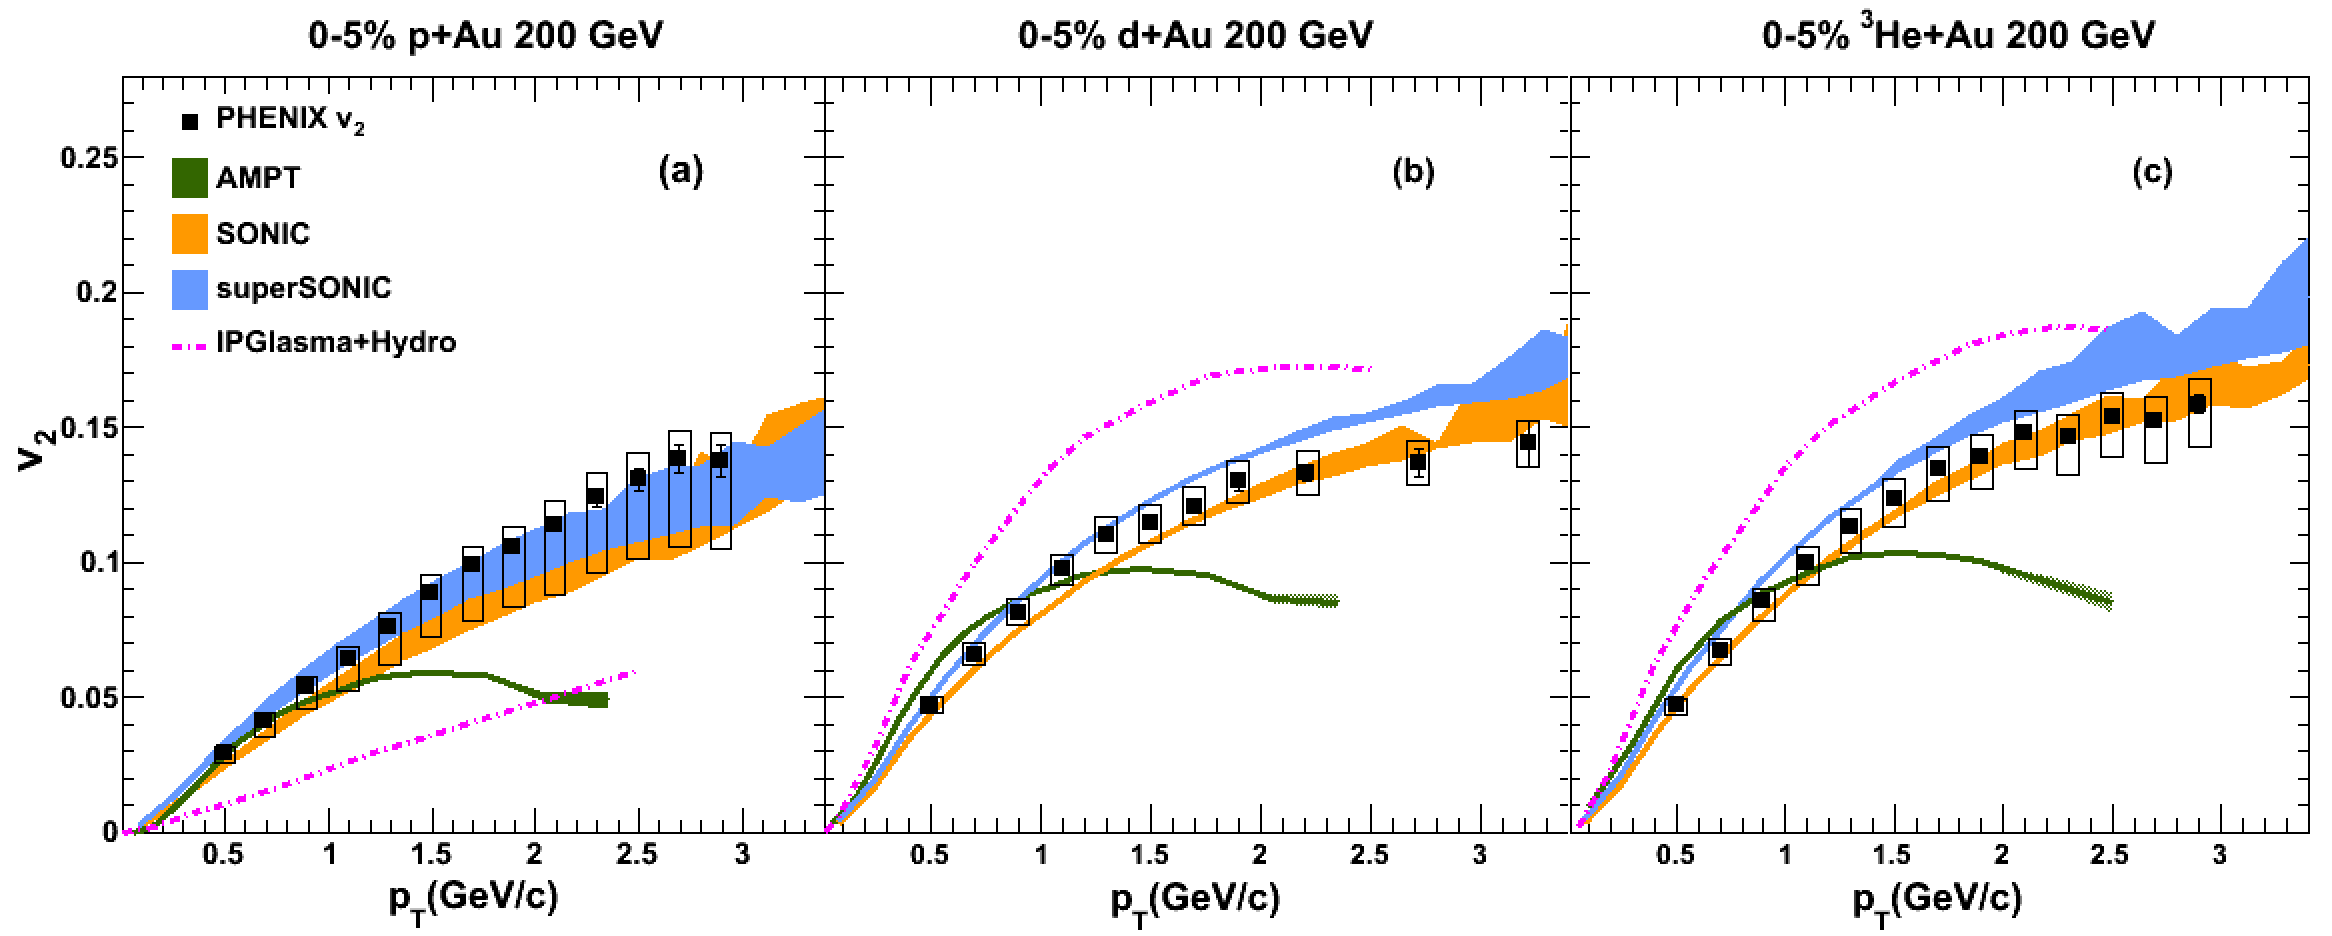
\includegraphics[width=1.0\linewidth]{figs/indepth_theory_comparison.png}
\caption{Transverse momentum dependence of $v_2$ in central 0-5\% (a) p+Au, (b) d+Au, and (c) He+Au collisions at \sqsn = 200 GeV. Theoretical calculations from AMPT, SUPERSONIC, and IPGlasma+Hydro are shown in each panel. Note that the data points shown include non-flow contributions, whose estimated magnitude is accounted for in the asymmetric systematic uncertainties.}
\label{fig:indepth_comp_three}
\end{center}
\end{figure}

These results impose strong constraints on any model attempting to describe
 small system collectivity, whether by the formation of strongly interacting hot nuclear matter, or by other mechanisms.
 We observe an imperfect scaling of $v_2$ with $\epsilon_2$, well reproduced by hydrodynamics, providing strong evidence for initial
 geometry as the source of final-state momentum anisotropy in these systems. This disfavors other explanations based
 on initial-state momentum space domain effects.